\usepackage{float}      
\usepackage{subcaption}
\section{Experiment 3: Multi-Modal Fusion (3D ResNet + Radiomics)}

\subsection{Rationale and Hypothesis}
The results from Experiment 2 (CT-Only) indicated that the 3D ResNet struggled to extract discriminative features from the voxel data alone, likely due to the limited sample size ($N=87$) relative to the high dimensionality of the input. 

To mitigate this, Experiment 3 introduces a Multi-Modal architecture. By integrating Radiomics, quantitative features describing tumor texture, intensity, and shape, we aim to provide the model with high-level, pre-engineered signals that can guide the deep learning feature extractor. The hypothesis is that the explicit radiomics features will stabilize training and improve classification performance for TTF1 and CK7.

\subsection{Methodology}

\subsubsection{Data Preparation}
The dataset remains the same 87-patient cohort with the stratified split used in Experiment 2. However, the input pipeline was modified to support dual inputs:
\begin{enumerate}
    \item \textbf{3D CT Volume:} Preprocessed as before (resized to $128\times128\times128$, intensity normalized).
    \item \textbf{Radiomics Vector:} A vector of 107 radiomics features (extracted via PyRadiomics). These features were standardized (Z-score normalization) using statistics derived strictly from the training set to prevent data leakage.
\end{enumerate}

\subsubsection{Dual-Stream Architecture}
A custom Keras model was constructed to process both data modalities simultaneously using a Late Fusion strategy:

\begin{itemize}
    \item \textbf{Stream 1 (Image Encoder):} The 3D ResNet body from Experiment 2 is used to map the input volume to a dense latent vector ($d_{img} = 128$).
    \item \textbf{Stream 2 (Tabular Encoder):} A Multi-Layer Perceptron (MLP) processes the radiomics vector.
    \begin{itemize}
        \item Layers: $Dense(64, ReLU) \rightarrow Dropout(0.3) \rightarrow Dense(32, ReLU)$.
        \item Output: A dense latent vector ($d_{rad} = 32$).
    \end{itemize}
    \item \textbf{Fusion Block:} The two latent vectors are concatenated to form a combined representation of the patient.
    \item \textbf{Classification Heads:} The fused vector feeds into two separate sigmoid output heads for \textbf{TTF1} and \textbf{CK7} prediction.
\end{itemize}

\subsection{Experimental Results}
\begin{figure}[H]
    \centering
    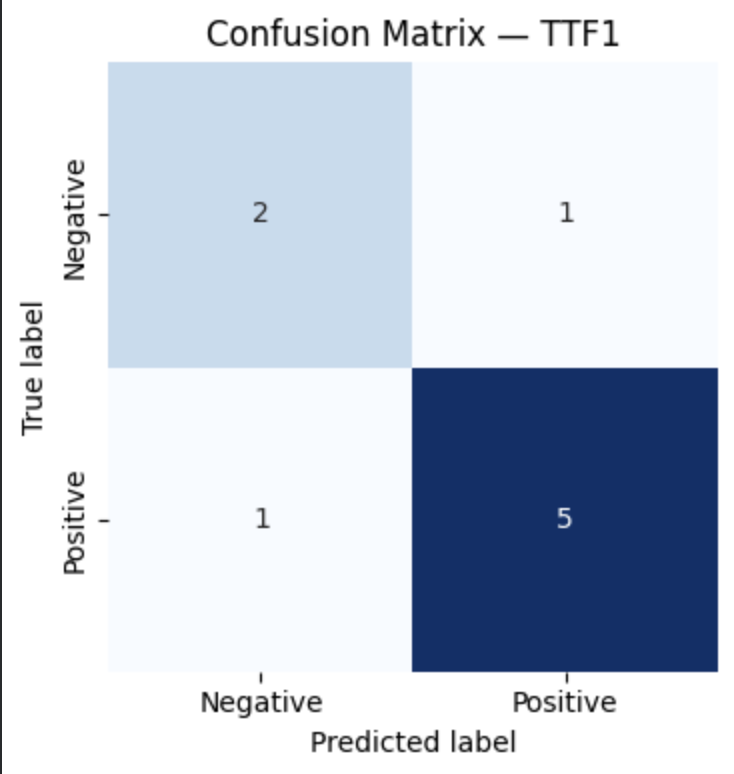
\includegraphics[width=0.5\textwidth]{Screenshot 2025-11-20 at 10.27.28.png}
    \caption{Confusion Matrix for TTF1.}
    \centering
    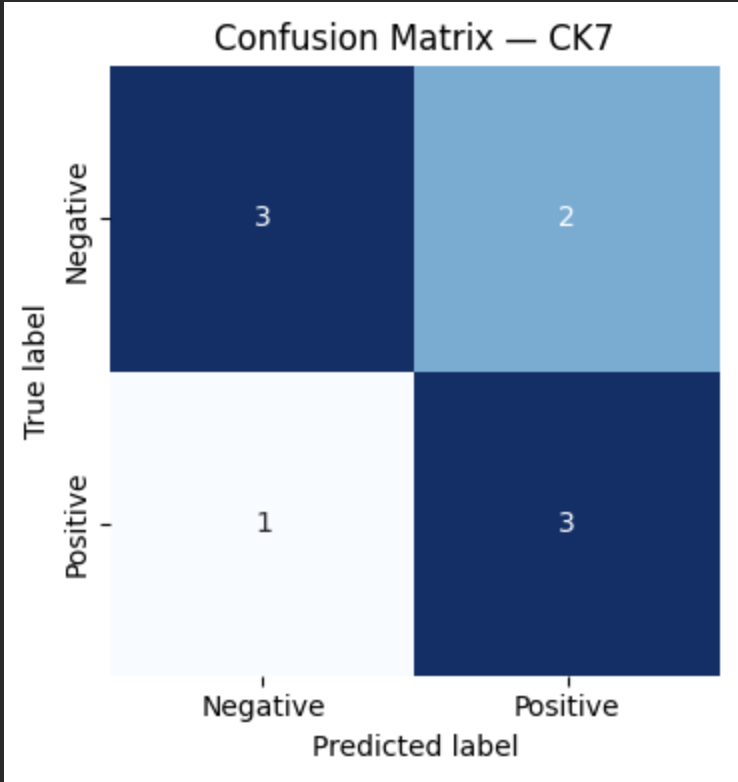
\includegraphics[width=0.5\textwidth]{Screenshot 2025-11-20 at 10.27.37.png}
    \caption{Confusion Matrix for CK7.}
\end{figure}

\subsubsection{Training Dynamics}
The model was trained using the Adam optimizer ($LR=1e-4$) for 100 epochs with early stopping. The inclusion of radiomics features resulted in faster convergence compared to the CT-only baseline, suggesting that the tabular features provided strong initial gradients.



\subsubsection{Test Set Metrics}
The multi-modal model demonstrated an improvement over the image-only baseline, particularly in distinguishing the minority classes.





\subsection{Conclusion of Experiment 3}
Fusing Radiomics with 3D CNN features proved to be a more effective strategy for this small-data regime. The engineered features acted as a "scaffold," allowing the model to make reasonable predictions even when the image features were ambiguous. This confirms that for limited medical imaging datasets, hybrid modeling outperforms pure deep learning approaches.